\documentclass[11pt,preprint, authoryear]{elsarticle}

\usepackage{lmodern}
%%%% My spacing
\usepackage{setspace}
\setstretch{1.2}
\DeclareMathSizes{12}{14}{10}{10}

% Wrap around which gives all figures included the [H] command, or places it "here". This can be tedious to code in Rmarkdown.
\usepackage{float}
\let\origfigure\figure
\let\endorigfigure\endfigure
\renewenvironment{figure}[1][2] {
    \expandafter\origfigure\expandafter[H]
} {
    \endorigfigure
}

\let\origtable\table
\let\endorigtable\endtable
\renewenvironment{table}[1][2] {
    \expandafter\origtable\expandafter[H]
} {
    \endorigtable
}


\usepackage{ifxetex,ifluatex}
\usepackage{fixltx2e} % provides \textsubscript
\ifnum 0\ifxetex 1\fi\ifluatex 1\fi=0 % if pdftex
  \usepackage[T1]{fontenc}
  \usepackage[utf8]{inputenc}
\else % if luatex or xelatex
  \ifxetex
    \usepackage{mathspec}
    \usepackage{xltxtra,xunicode}
  \else
    \usepackage{fontspec}
  \fi
  \defaultfontfeatures{Mapping=tex-text,Scale=MatchLowercase}
  \newcommand{\euro}{€}
\fi

\usepackage{amssymb, amsmath, amsthm, amsfonts}

\def\bibsection{\section*{References}} %%% Make "References" appear before bibliography


\usepackage[round]{natbib}

\usepackage{longtable}
\usepackage[margin=2.3cm,bottom=2cm,top=2.5cm, includefoot]{geometry}
\usepackage{fancyhdr}
\usepackage[bottom, hang, flushmargin]{footmisc}
\usepackage{graphicx}
\numberwithin{equation}{section}
\numberwithin{figure}{section}
\numberwithin{table}{section}
\setlength{\parindent}{0cm}
\setlength{\parskip}{1.3ex plus 0.5ex minus 0.3ex}
\usepackage{textcomp}
\renewcommand{\headrulewidth}{0.2pt}
\renewcommand{\footrulewidth}{0.3pt}

\usepackage{array}
\newcolumntype{x}[1]{>{\centering\arraybackslash\hspace{0pt}}p{#1}}

%%%%  Remove the "preprint submitted to" part. Don't worry about this either, it just looks better without it:
\makeatletter
\def\ps@pprintTitle{%
  \let\@oddhead\@empty
  \let\@evenhead\@empty
  \let\@oddfoot\@empty
  \let\@evenfoot\@oddfoot
}
\makeatother

 \def\tightlist{} % This allows for subbullets!

\usepackage{hyperref}
\hypersetup{breaklinks=true,
            bookmarks=true,
            colorlinks=true,
            citecolor=blue,
            urlcolor=blue,
            linkcolor=blue,
            pdfborder={0 0 0}}


% The following packages allow huxtable to work:
\usepackage{siunitx}
\usepackage{multirow}
\usepackage{hhline}
\usepackage{calc}
\usepackage{tabularx}
\usepackage{booktabs}
\usepackage{caption}


\newenvironment{columns}[1][]{}{}

\newenvironment{column}[1]{\begin{minipage}{#1}\ignorespaces}{%
\end{minipage}
\ifhmode\unskip\fi
\aftergroup\useignorespacesandallpars}

\def\useignorespacesandallpars#1\ignorespaces\fi{%
#1\fi\ignorespacesandallpars}

\makeatletter
\def\ignorespacesandallpars{%
  \@ifnextchar\par
    {\expandafter\ignorespacesandallpars\@gobble}%
    {}%
}
\makeatother

\newenvironment{CSLReferences}[2]{%
}

\urlstyle{same}  % don't use monospace font for urls
\setlength{\parindent}{0pt}
\setlength{\parskip}{6pt plus 2pt minus 1pt}
\setlength{\emergencystretch}{3em}  % prevent overfull lines
\setcounter{secnumdepth}{5}

%%% Use protect on footnotes to avoid problems with footnotes in titles
\let\rmarkdownfootnote\footnote%
\def\footnote{\protect\rmarkdownfootnote}
\IfFileExists{upquote.sty}{\usepackage{upquote}}{}

%%% Include extra packages specified by user

%%% Hard setting column skips for reports - this ensures greater consistency and control over the length settings in the document.
%% page layout
%% paragraphs
\setlength{\baselineskip}{12pt plus 0pt minus 0pt}
\setlength{\parskip}{12pt plus 0pt minus 0pt}
\setlength{\parindent}{0pt plus 0pt minus 0pt}
%% floats
\setlength{\floatsep}{12pt plus 0 pt minus 0pt}
\setlength{\textfloatsep}{20pt plus 0pt minus 0pt}
\setlength{\intextsep}{14pt plus 0pt minus 0pt}
\setlength{\dbltextfloatsep}{20pt plus 0pt minus 0pt}
\setlength{\dblfloatsep}{14pt plus 0pt minus 0pt}
%% maths
\setlength{\abovedisplayskip}{12pt plus 0pt minus 0pt}
\setlength{\belowdisplayskip}{12pt plus 0pt minus 0pt}
%% lists
\setlength{\topsep}{10pt plus 0pt minus 0pt}
\setlength{\partopsep}{3pt plus 0pt minus 0pt}
\setlength{\itemsep}{5pt plus 0pt minus 0pt}
\setlength{\labelsep}{8mm plus 0mm minus 0mm}
\setlength{\parsep}{\the\parskip}
\setlength{\listparindent}{\the\parindent}
%% verbatim
\setlength{\fboxsep}{5pt plus 0pt minus 0pt}



\begin{document}



\begin{frontmatter}  %

\title{Question 1}

% Set to FALSE if wanting to remove title (for submission)




\author[Add1]{Ronan Morris}
\ead{22876634}





\address[Add1]{Stellenbosch University}



\vspace{1cm}





\vspace{0.5cm}

\end{frontmatter}

\setcounter{footnote}{0}



%________________________
% Header and Footers
%%%%%%%%%%%%%%%%%%%%%%%%%%%%%%%%%
\pagestyle{fancy}
\chead{}
\rhead{}
\lfoot{}
\rfoot{\footnotesize Page \thepage}
\lhead{}
%\rfoot{\footnotesize Page \thepage } % "e.g. Page 2"
\cfoot{}

%\setlength\headheight{30pt}
%%%%%%%%%%%%%%%%%%%%%%%%%%%%%%%%%
%________________________

\headsep 35pt % So that header does not go over title




\hypertarget{artificial-intelligence-or-active-management}{%
\section{Artificial Intelligence or Active
Management?}\label{artificial-intelligence-or-active-management}}

For this question, I decided to focus on only dates after the global
financial crisis. Firstly, the funds had different starting days and I
wanted only funds that had existed for the entire time that the AI Fund
had existed, so as to be able to meaningfully compare returns. I also
thought that in a question about volatility and returns, it would be
more fair to only look at the performance of different funds after the
GFC. I also did not select all funds in the data set. For actively
managed funds, I selected the best and worst performing funds over the
time period (measured by average returns). I did the same methodology
for Indices.

Below you find the distribution of returns for three funds. The S1007 is
the best performing actively managed fund in this regard, whereas the
V412 is the worst. It is pivotal to mention that these returns are fees
adjusted for the actively managed funds (estimated as 2.5\% annualized).
From this plot, we can see that the AI Fund outperforms the worst
performing actively managed fund, while having a similar return
distribution to the S1007. The S1007 does have a fatter tail on the high
end, but it also faces more losses. The AI Fund also is more likely to
yield mid-high level returns than either fund, it only lacks in extreme
(high risk) regions.

\begin{figure}[H]

{\centering 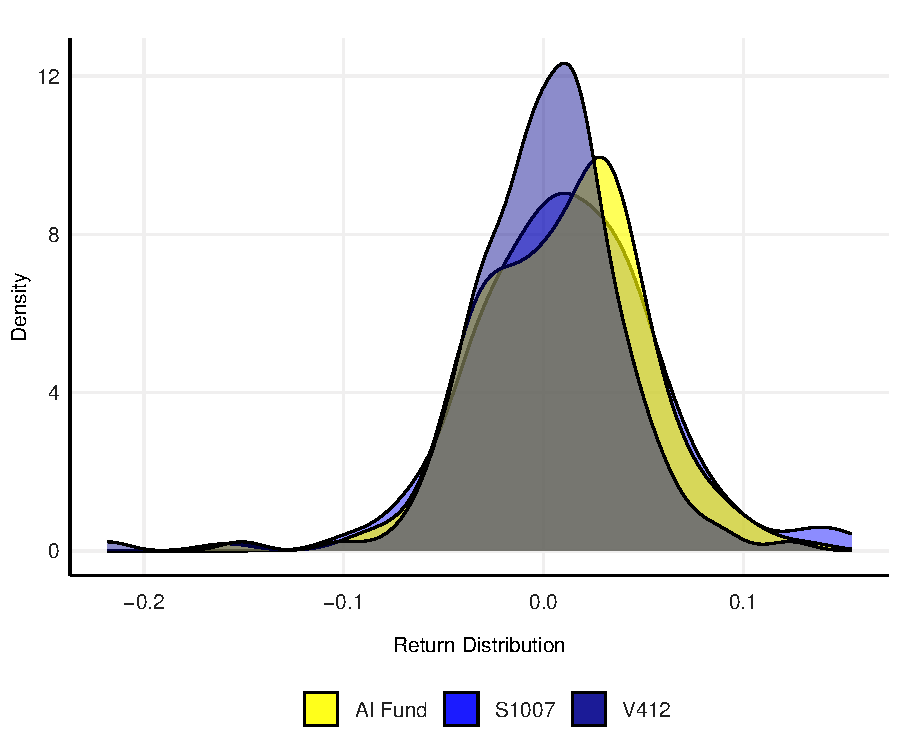
\includegraphics{Question-1_files/figure-latex/unnamed-chunk-1-1} 

}

\caption{ \label{Figure1.1}}\label{fig:unnamed-chunk-1}
\end{figure}

The AI Fund could not outperform Indices. It has a similar return
distribution to the ``worst'' index fund. It performs visibly worse than
the best Index fund, even though these have been capped (1\%
annualized).

\begin{figure}[H]

{\centering \includegraphics{Question-1_files/figure-latex/unnamed-chunk-2-1} 

}

\caption{ \label{Figure1.2}}\label{fig:unnamed-chunk-2}
\end{figure}

The AI Fund also has an incredibly similar returns distribution to the
Capped SWIX, which is the benchmark return series for this study. It
does have fatter tails, or rather, more extreme values, but this is paid
off by the potential for slightly higher returns than the benchmark.

\begin{figure}[H]

{\centering \includegraphics{Question-1_files/figure-latex/unnamed-chunk-3-1} 

}

\caption{ \label{Figure1.3}}\label{fig:unnamed-chunk-3}
\end{figure}

Out of the selected funds (the benchmark, the best and worst Index, and
best and worst Actively managed fund), the AI Fund performs the second
best. This cumulative return plot did not account for fees, however. The
AI Fund consistently outperforms the benchmark rate. Notice that active
management might seem attractive due to the presence of the best
performing fund as one that is active, but the worst performing fund is
also one which is active. I argue that the AI Fund offers a far better
risk adjusted return.

\begin{figure}[H]

{\centering \includegraphics{Question-1_files/figure-latex/unnamed-chunk-5-1} 

}

\caption{ \label{Figure1.4}}\label{fig:unnamed-chunk-5}
\end{figure}

In terms of rolling average returns (3 year), one could still argue that
the AI Fund is the second best performing, with large periods of time
outperforming the benchmark rate, and either outperforming, or
performing similarly, to other funds. Once again, active management has
the best (and worst) return, which is a large risk to take.

\begin{figure}[H]

{\centering \includegraphics{Question-1_files/figure-latex/unnamed-chunk-6-1} 

}

\caption{ \label{Figure1.5}}\label{fig:unnamed-chunk-6}
\end{figure}

If you look at the rolling standard deviation (3 year), the point about
risk is exhibited excellently. Since 2020, both the best and worst
actively managed fund have had higher levels of volatility than the AI
Fund. The AI fund has passed the COVID volatility hurdle with incredibly
consistency, maintaining a lower volatility than even the benchmark at
times.

\begin{figure}[H]

{\centering \includegraphics{Question-1_files/figure-latex/unnamed-chunk-7-1} 

}

\caption{ \label{Figure1.6}}\label{fig:unnamed-chunk-7}
\end{figure}

\bibliography{Tex/ref}





\end{document}
